\documentclass{sigchi}


% Load basic packages
\usepackage{balance}  % to better equalize the last page
\usepackage{graphics} % for EPS, load graphicx instead
\usepackage{times}    % comment if you want LaTeX's default font
\usepackage{url}      % llt: nicely formatted URLs
\usepackage{tabularx}

% llt: Define a global style for URLs, rather that the default one
\makeatletter
\def\url@leostyle{%
  \@ifundefined{selectfont}{\def\UrlFont{\sf}}{\def\UrlFont{\small\bf\ttfamily}}}
\makeatother
\urlstyle{leo}


% To make various LaTeX processors do the right thing with page size.
\def\pprw{8.5in}
\def\pprh{11in}
\special{papersize=\pprw,\pprh}
\setlength{\paperwidth}{\pprw}
\setlength{\paperheight}{\pprh}
\setlength{\pdfpagewidth}{\pprw}
\setlength{\pdfpageheight}{\pprh}

% Make sure hyperref comes last of your loaded packages, 
% to give it a fighting chance of not being over-written, 
% since its job is to redefine many LaTeX commands.
\usepackage[pdftex]{hyperref}
\hypersetup{
pdftitle={SIGCHI Conference Proceedings Format},
pdfauthor={LaTeX},
pdfkeywords={SIGCHI, proceedings, archival format},
bookmarksnumbered,
pdfstartview={FitH},
colorlinks,
citecolor=black,
filecolor=black,
linkcolor=black,
urlcolor=black,
breaklinks=true,
}

% create a shortcut to typeset table headings
\newcommand\tabhead[1]{\small\textbf{#1}}


% End of preamble. Here it comes the document.
\begin{document}

\title{Pervasive Project}
\subtitle{The ITU Context Phone Platform}

\numberofauthors{3}
\author{
  \alignauthor Ivan Naumovski\\
    \email{inau@itu.dk}\\
  \alignauthor Martino Secchi\\
    \email{msec@itu.dk}\\
  \alignauthor Diem Hoang Nguyen\\
    \email{hong@itu.dk}\\
}

\maketitle

\begin{abstract}
The project's objective is that to create a pervasive cloud-based context-aware system. 
The system created is based on two technologies: an Android application for smartphones that can sense context data, and a cloud-based infrastructure, based on Google App Engine, that stores such information in correlation to its physical location.
\end{abstract}

\keywords{
Pervasive Computing, Context Aware, Smartphone, Networking, Google App Engine, Android Sensors}

\category{H.5.m.}{Information interfaces and presentation (e.g., HCI)}{Miscellaneous}

\section{Introduction}
This report is part of the first mandatory assignment in the course Pervasive Computing at the IT-University of Copenhagen (ITU), relating to the subject of context aware systems \cite{Schilit:1994:CACA}.
 The purpose of this project is to create a mobile application for Android, supported by ITU iBeacon infrastructure and by a  cloud based service, able to sense, store, and show context information about geographic locations. 
 
 \section{System Description}

The system is composed of four major components:
\begin{itemize}
\item the map activity
\item the ibeacon scanner
\item the context service
\item the cloud based infrastructure
\end{itemize}
The system has been designed to work over the existing iBeacon infrastructure of IT University, recognising automatically the iBeacons used in the building.

\textbf{Map Activity.} The map activity is responsible of locating the user's position and displaying it to a map.  On the map the user of the application can see the positions of iBeacons that are known to the system. The iBeacon that is closest to the user is displayed in green, while the others are grey. Every beacon has some context informations attached, that can also be viewed on the map by clicking on the map marker.\\

\begin{figure}[!h]
\centering
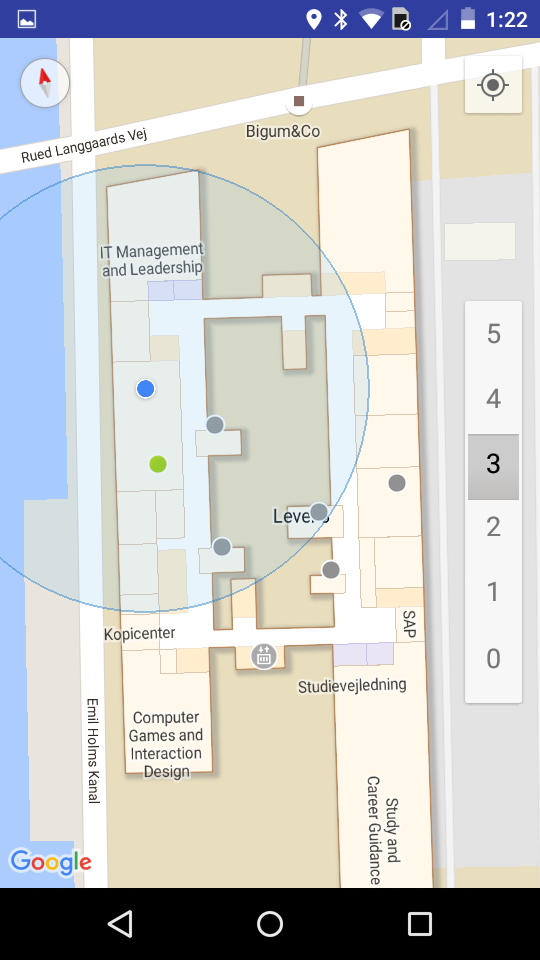
\includegraphics[width=0.3\columnwidth]{images/figure1}
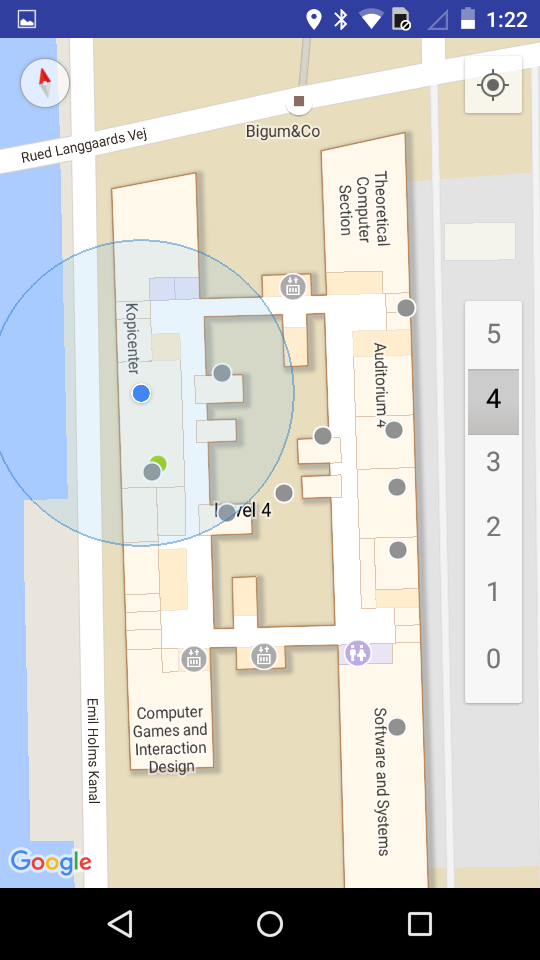
\includegraphics[width=0.3\columnwidth]{images/figure2}
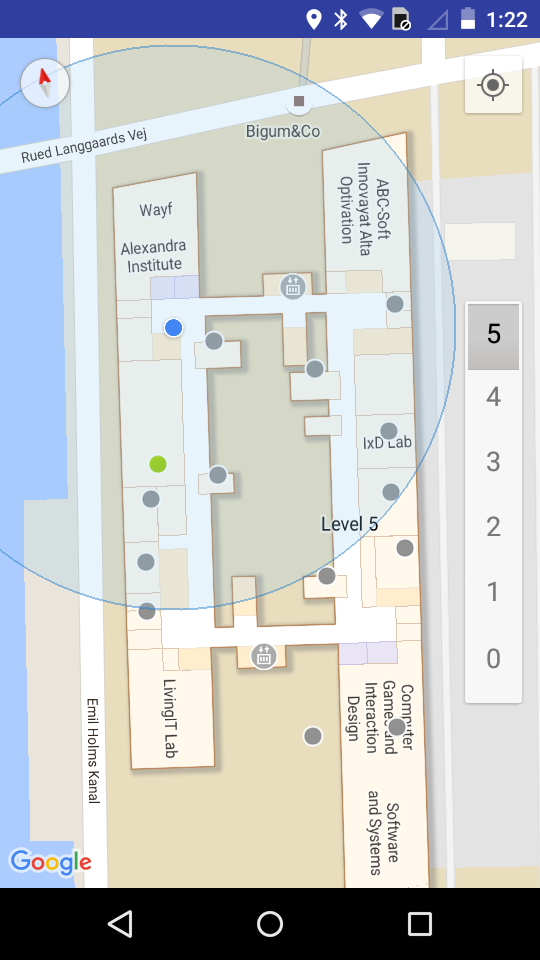
\includegraphics[width=0.3\columnwidth]{images/figure3}
\caption{The user location and the iBeacons position are displayed on the map.
It is also possible to select the different floor levels from the building.}
\label{fig:figure2}
\end{figure}

\textbf{iBeacon scanner.} The iBeacon scanner is activated by the user, and uses Bluetooth Low Energy technology to scan for iBeacons near the device. The found beacons are then displayed to the user on list, but only in case they are not known to the system. At this point it is the user choice to store their information on the system, providing a custom location by long pressing on the map. \\
\textbf{Context Service.} The context service runs in the background of the map activity, and is responsible of collecting context information about the user's location and send it to the cloud infrastructure. The entire process is automated and doesn't require the user's interaction. \\
The context information obtained is of three types: atmospheric pressure, ambient temperature, and level of sound. This informations are supposed to support the student-user in decisions he may face that involve knowledge of the surrounding environment. For example, information about sound or temperature may help one decide wether some place is ideal for studying, while atmospheric pressure could be used, by the user himself or by some other service, to  determine weather conditions and likelihood of rain. \\

\begin{figure}[!h]
\centering
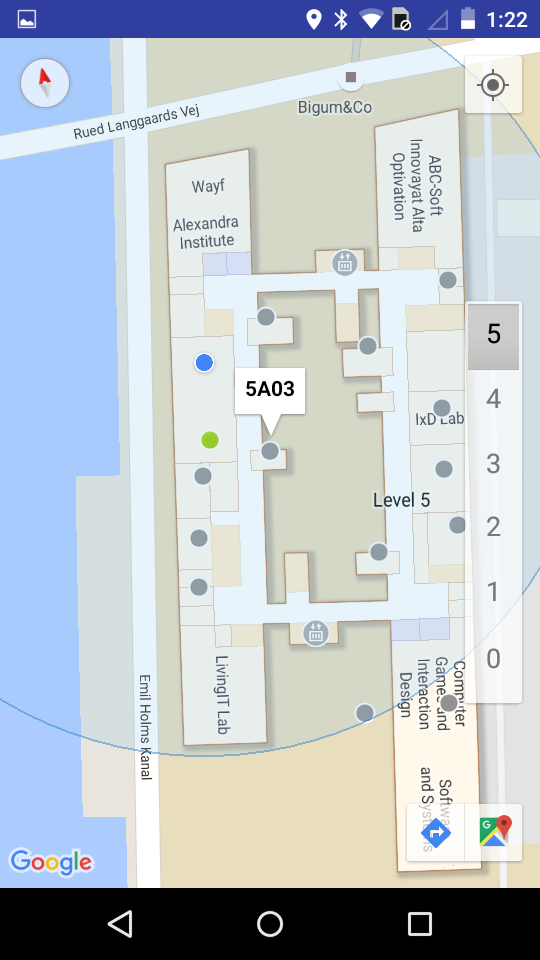
\includegraphics[width=0.3\columnwidth]{images/figure4}
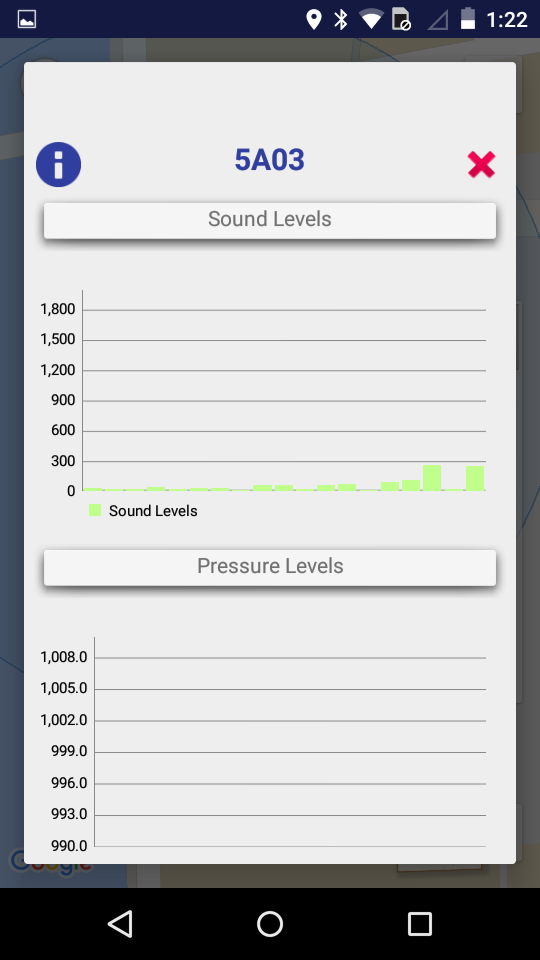
\includegraphics[width=0.3\columnwidth]{images/figure5}
\caption{Context information is displayed when clicking on the location.}
\label{fig:figure1}
\end{figure}

\textbf{Cloud Based Infrastructure. }  A cloud based storage system is been developed using Google App Engine, that implements CRUD operations on beacon and context information based on REST requests.

\section{Technical Implementation}
\subsection{The Cloud}
We are using the Google App Engine to host our cloud, and we use their DataStorage API for persistance(Objectify is the ORM framework we use).

We had a thorough discussion on how exactly beacons and context information should be linked together, we settled on having two tables with no foreign key mappings.\\
One table for beacon data and one table for context information.\\

The beacon table is as follows:
\begin{quotation}
\textbf{Beacon}(\underline{key}, uid, major, minor, lat, lng, updated);
\end{quotation}
The key is generated as a combination of the uid, major and minor values, even though there is some redundancy when doing so.

The context table is as follows:
\begin{quotation}
\textbf{Context}(\underline{uid}, type, values, lat, lng, updated);
\end{quotation}
The idea is that a single location can have multiple contexts. This is due to the fact that the sensors we have chosen make more sense when we can track values over time (sound and pressure).
This would not have been possible if only one context existed per beacon.

The idea is that we select contexts for a specific location and present their change in values over time or do some notifications based on the change in values.

%The approach we went with is using the sensed beacons(not to be mistaken with the stored beacon entities) to pinpoint the closest beacon.

%Once the closest beacon has been detected, we look it up in our local cache - if the beacon is not in the local SQLite instance, we look for it in the cloud.

%In case it doesnt exist in the cloud, we create one using the cloud API, this will respond with the freshly created entity as a result, which is then stored in the local SQLite instance.

We have built two java servlets supporting CRUD functionality one for beacons and one for contexts.

They expose the following HTML request types - GET, POST and DELETE.

GET is for retrieval of data, POST is for either creation or merging of data, while DELETE is for deletion of data.

GET and DELETE expect query parameters, while POST expects a payload(body).

\subsubsection{Hosting}
The webserver is hosted at \textit{http://contextphone.appspot.com/}, the index page presents data currently in the datastore, and some information about the API.

The REST API is hosted at the path 'r/', and each sub table has its corresponding subpath.
\textit{http://contextphone.appspot.com/r/contexts}\\
\textit{http://contextphone.appspot.com/r/beacons}

\subsubsection{API cheatsheet}

\textbf{Contexts}


\begin{tabularx}{.5\textwidth}{  p{.1\textwidth}X }
\textbf{GET} & \textbf{Query keys:} lat, lng, after, uid\\
 & for getting contexts at (2,2) after 1.2.2015 use \textbf{'?lat=2\&lng=2\&after=1420156800000'}\\
 & for getting a single context use \textbf{'?uid=12345678'} to get context with uid 12345678\\
\textbf{POST} & d\\
\textbf{DELETE} & f\\
\end{tabularx}

\subsection{Context Monitoring}

The process of monitoring the context information happens in the background, without involving the user. \\
All the monitoring is handled by a service on the mobile device of the user, that starts and works behind the map activity.
As already stated, the collected context information is of three types: atmospheric pressure, ambient temperature, and level of sound. \\
Atmospheric pressure is measured in hPa (millibar) and ambient temperature in degree Celsius.
Sound measurements are calibrated depending on the device, and results may vary.
Each type has its own context monitor that runs on its own thread. \\
The detections are performed once every a fixed interval of time (one minute in the current implementation), and only if/when possible. In fact, not all modern devices are equipped with pressure or temperature sensors, and in those cases the monitoring would not be possible for the specific types.\\
The sound monitor records sound through the device's microphone over short intervals of time, then computes the average sound amplitude. This operation is repeated every minute. \\
Once that the context information is available, it is sent to the web service together with the location where that information was recorded (the user location).

\subsection{Beacon Mapping}
The Beacon is a proximity-based location using the Bluetooth discovery protocol.
Typically, an iBeacon can transmits Universally Unique Identifier (UUID), Major, Minor, Distance from the device to the Beacon, Received Signal Strength Indicator (RSSI), etc.
In order to detect the Beacon, the Android device should support Bluetooth Low Energy (BLE) and Android 4.3+.
We use Android Beacon Library which provide APIs to interact with Beacons, specifically for monitoring and ranging iBeacons nearby.

The location of Beacons at ITU will be calculated by Major and Minor information.
The Major indicates the floor and the Minor shows the area and room number.
For example, with Major = 3 and Minor = 1221, the Beacon will locate at floor 3, 'A' area and room number 22.
Because every ITU iBeacon will be installed in one specific room so we use the GPS coordinates of the room to indicate the location of the iBeacon.
For obtaining the ITU room location, we manually place a marker on Google Map at the position of the room to get its latitude and longitude value. 

During scanning process, the android device will check if the current Beacon was stored on server or not by finding on database using its key.
The iBeacon key is the combination of UUID, Major and Minor.
To do that, we send a GET request to server with information is a key of the iBeacon.
The responses from server will tell us if the Beacon was stored or not.
If the iBeacon is not stored,we will store it by sending a POST request to server with the information of the iBeacon including UUID, Major, Minor, Latitude and Longitude.

To find the closest iBeacon, we iterate through the list of available iBeacons to calculate the iBeacon that has the smallest distance to the Android device. After that, we show the position of closest iBeacon and current position of user together on Google Map.

There are many methods for estimating the current location: GPS, Assisted GPS, cell towers and Wi-Fi fingerprint.
Each provider has its own advantages and limitation, for example: GPS provides high precision but low speed and consumes more power while using Wi-Fi we receive medium precision but the process is faster and devices consume less power \cite{LaMarca:2008:LS, Constandache:2010:TMPLWWD}.
In this assignment, we combine these providers in order to make the location estimation more accurate as well as to utilize the advantages of such providers together. 
\section{Discussion}


% Balancing columns in a ref list is a bit of a pain because you
% either use a hack like flushend or balance, or manually insert
% a column break.  http://www.tex.ac.uk/cgi-bin/texfaq2html?label=balance
% multicols doesn't work because we're already in two-column mode,
% and flushend isn't awesome, so I choose balance.  See this
% for more info: http://cs.brown.edu/system/software/latex/doc/balance.pdf
%
% Note that in a perfect world balance wants to be in the first
% column of the last page.
%
% If balance doesn't work for you, you can remove that and
% hard-code a column break into the bbl file right before you
% submit:
%
% http://stackoverflow.com/questions/2149854/how-to-manually-equalize-columns-
% in-an-ieee-paper-if-using-bibtex
%
% Or, just remove \balance and give up on balancing the last page.
%
\balance

% If you want to use smaller typesetting for the reference list,
% uncomment the following line:
% \small
\bibliographystyle{acm-sigchi}
\bibliography{ubicomp}
\section{Appendix}

\end{document}
